%% Cartoon
\begin{figure}[h]
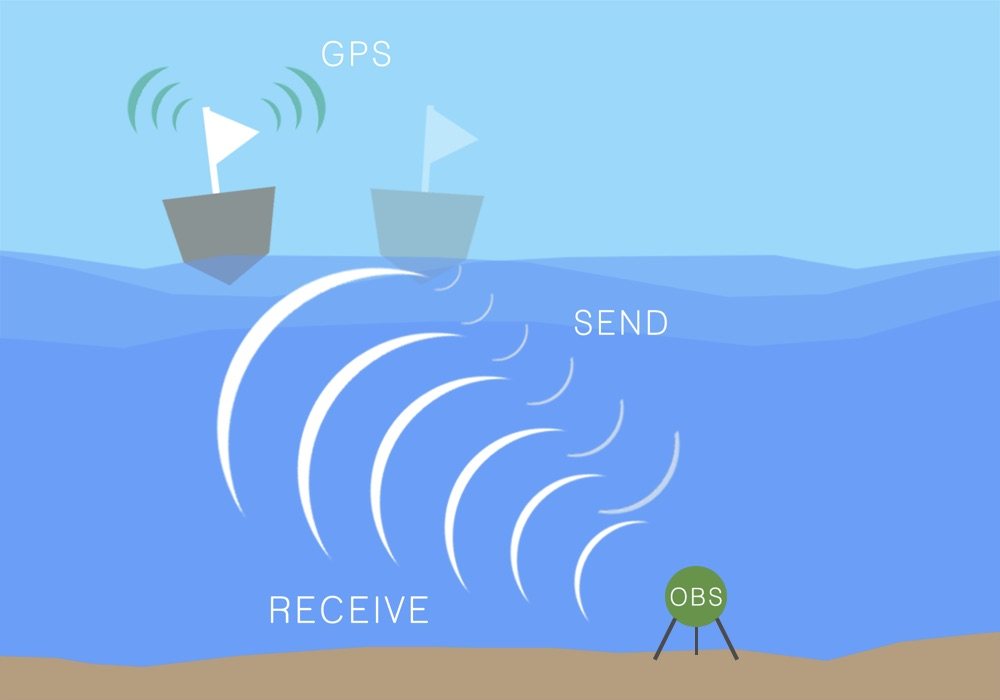
\includegraphics[trim=0cm 0cm 0cm 0cm,clip=true,width=\columnwidth]{OBS_Illustration.jpg}
\caption{Schematic of the acoustic ranging procedure. A 12~kHz acoustic pulse is sent from ship to OBS. After a time $\tau$, the OBS returns the acoustic signal to the ship at its new position. The difference in these send- and receive-times is referred to as the \textit{``Doppler''} correction, $\delta T$. From this schematic, it is clear that only ship tracks traveling toward or away from the instrument will result in a non-zero $\delta T$.}
\label{fig:cartoon}
\end{figure}

\newpage

%% Synthetic test (1-station) 
\begin{figure}[h]
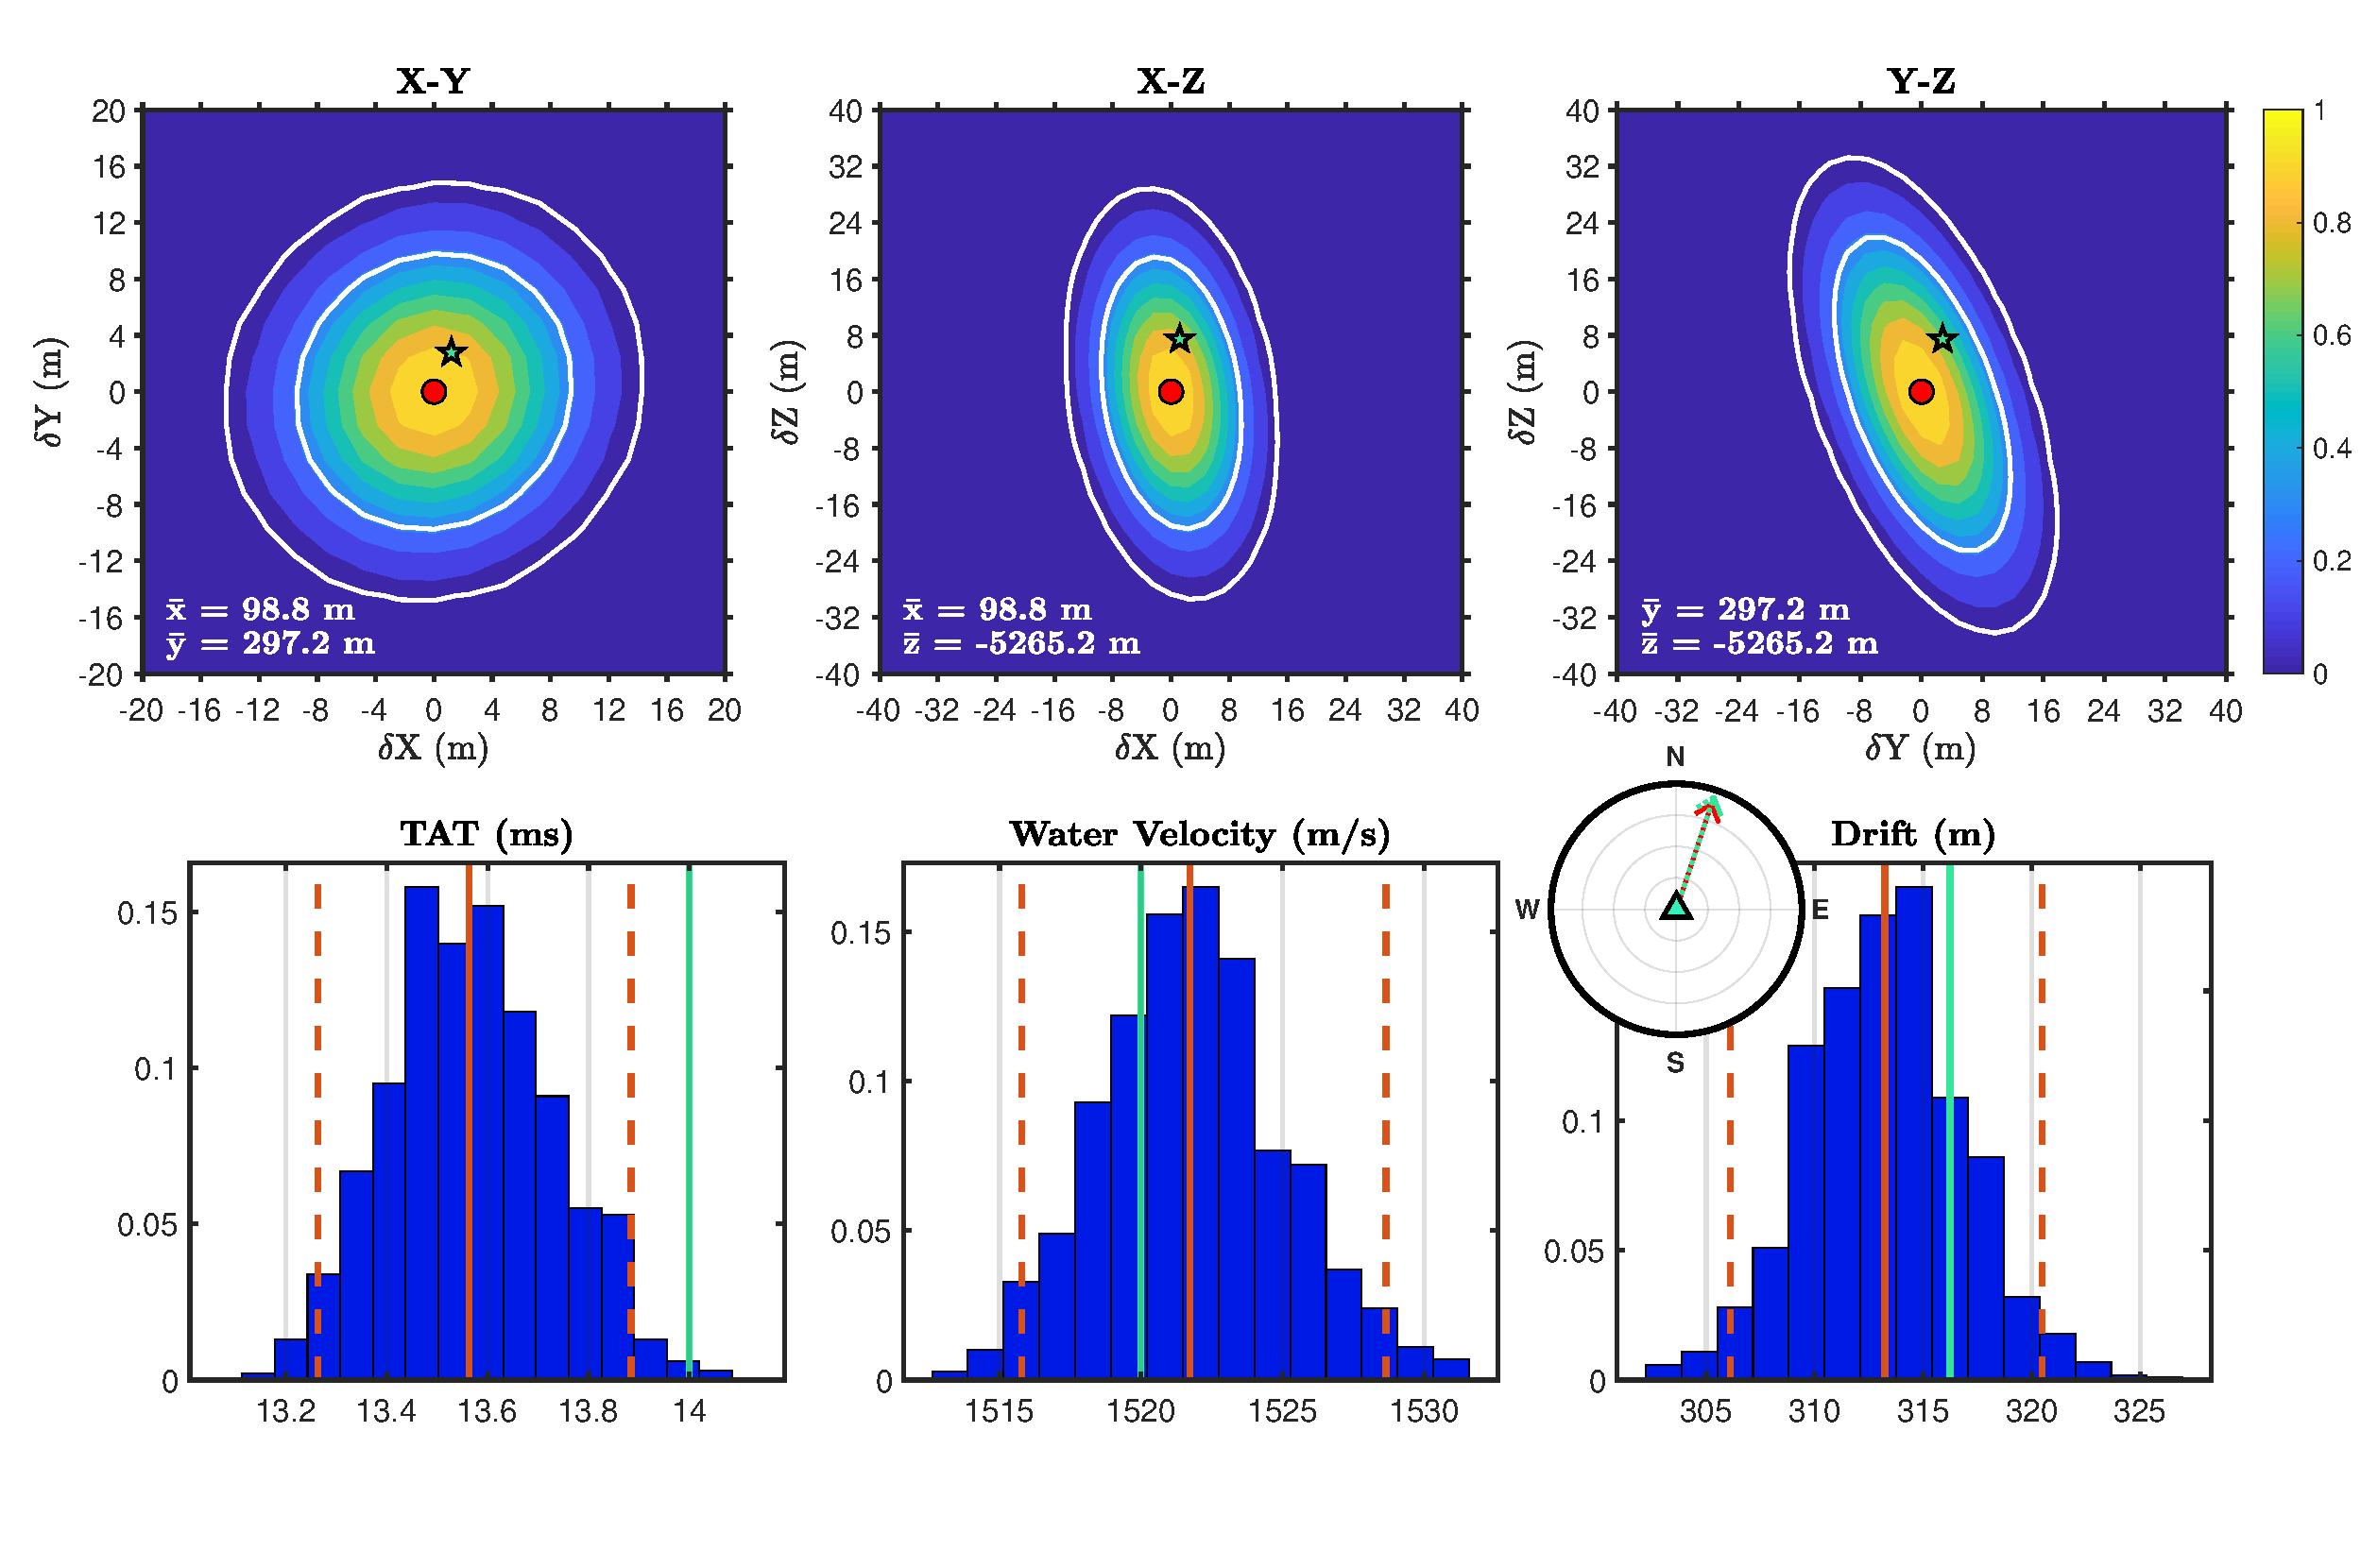
\includegraphics[trim=0cm 0cm 0cm 0cm,clip=true,width=\columnwidth]{Figure01.pdf}
\caption{Test of location algorithm using synthetic data calculated for a station at 5000~m depth using the \textit{PACMAN} geometry. a) The \textit{PACMAN} survey pattern colored by travel-time residuals. The gray and red squares represent the drop location and final inversion, respectively. The green star denotes the true location. b-c) Bootstrap histograms from a bootstrap analysis with 95th percentile values indicated by dashed red lines and the true value in green. Inset shows the direction of true (green dashed) and estimated (red) drift with respect to the starting location. d-f) Slices through the F-test surface with white lines showing 68\% and 95\% confidence. Symbols are the same as a). Comparison of the true input values with the inverted model parameters demonstrates that the location, depth, and water velocity are extremely well recovered, and the estimated uncertainties on these parameters are consonant with the actual misfit.}
\label{fig:one_sta_synth}
\end{figure}

\newpage

%% Comparison to previous tools
\begin{figure}[h]
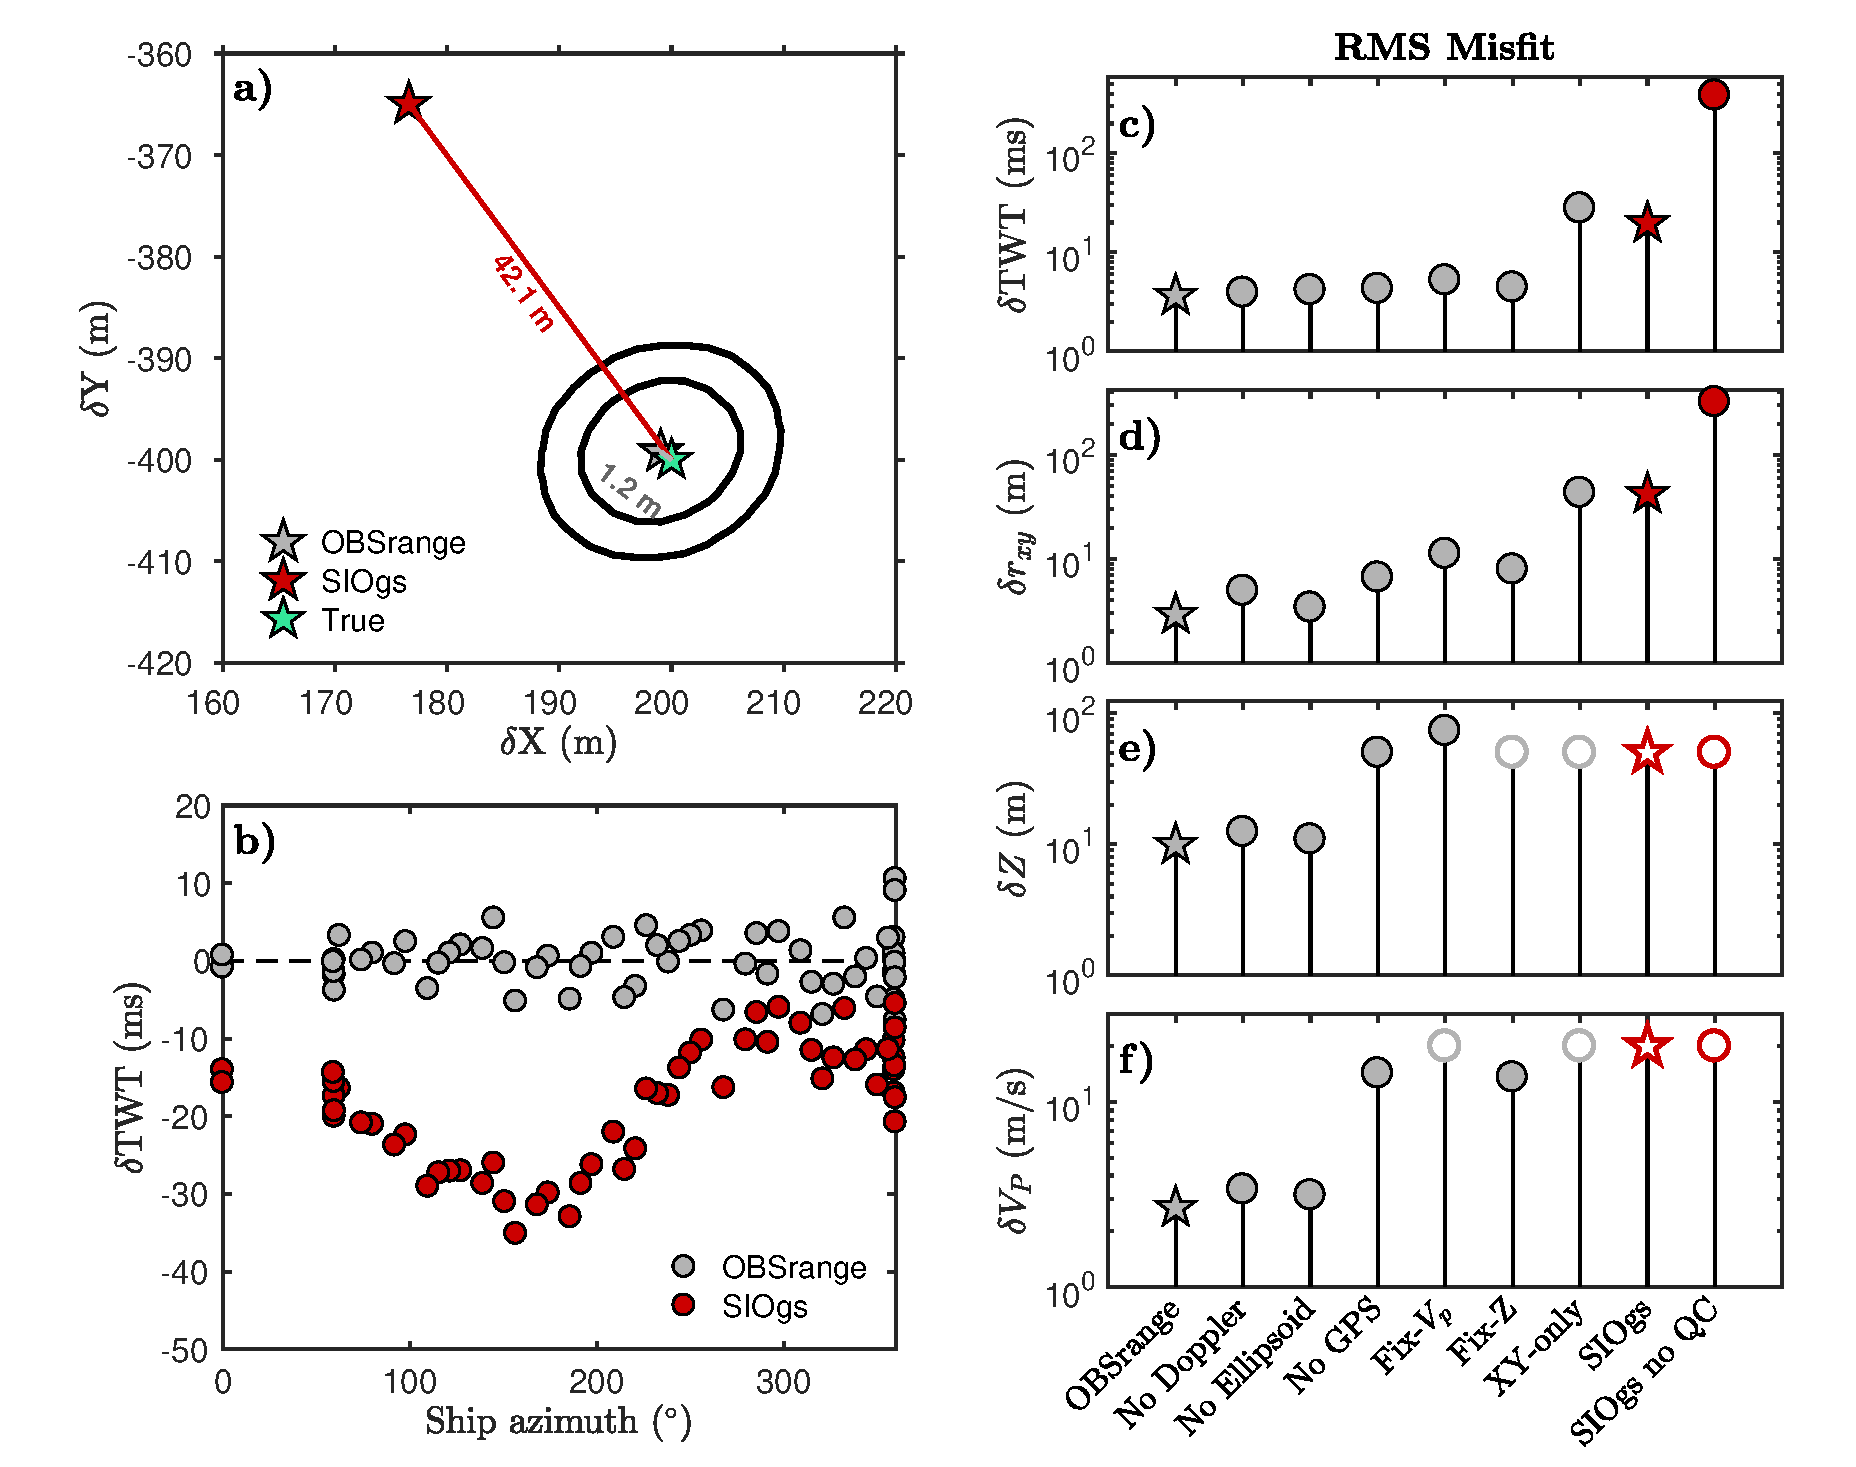
\includegraphics[trim=0cm 0cm 0cm 0cm,clip=true,width=\columnwidth]{Figure05.pdf}
\caption{ Synthetic test of OBSrange performance (gray symbols) compared with the SIO tool (red symbols) for a \textit{PACMAN} survey of radius 1 Nm at 5050~m depth. a) Map view comparing the OBSrange and SIOgs inverted instrument locations with the true location in green. Black contours show the 68\% and 95\% confidence from the OBSrange F-test. b) Two-way travel time (TWT) residuals for both methods as a function of ship azimuth from the true station location. c) TWT and d--f) model parameter RMS misfits for the 9 inversions, where closed symbols represent parameters that are solved for in the inversion and open symbols are parameters that remain fixed throughout the inversion. The horizontal instrument location misfit is given by $\delta r_{xy} = \sqrt{\delta x^2 + \delta y^2} $. Stars in c--f mark the inversion results shown in a) and b). See table~\ref{table:compare_tool} for details of each inversion.}
\label{fig:compare_tool}
\end{figure}

\newpage

%% Exploring survey geometries
\begin{figure}[h]
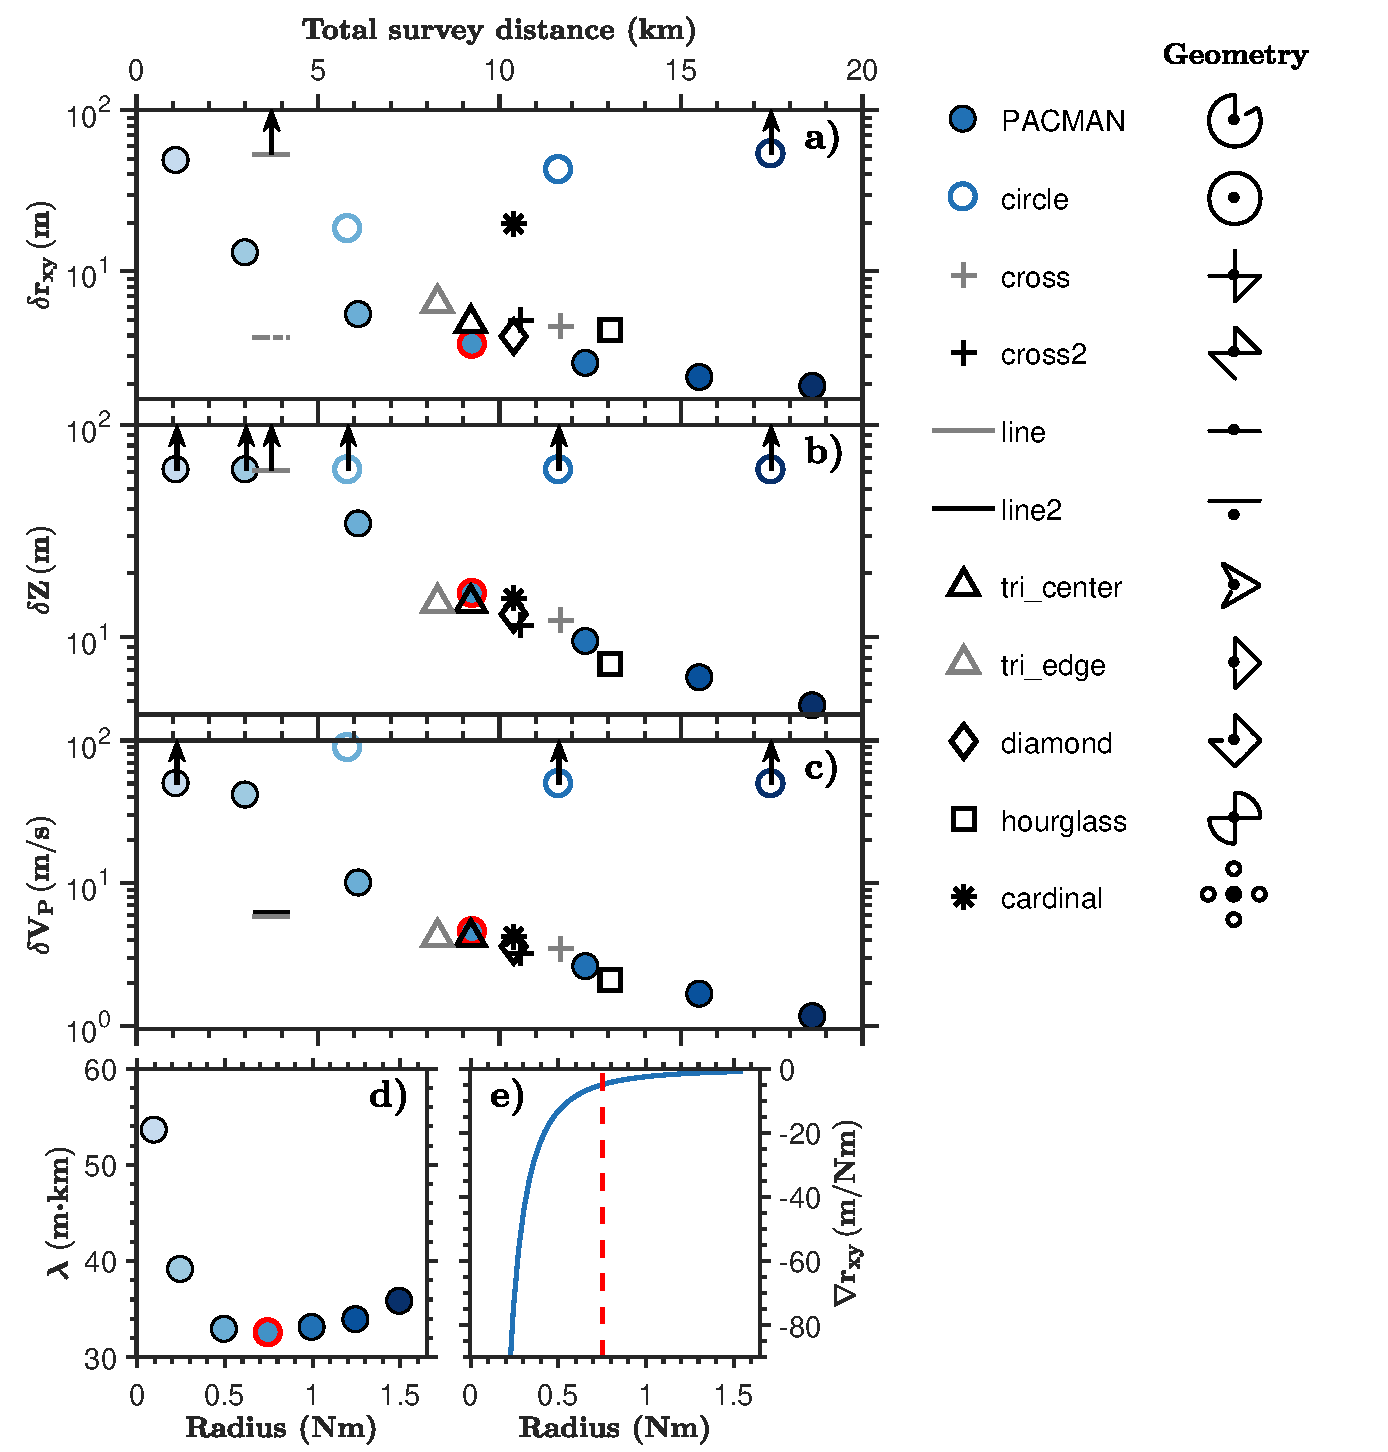
\includegraphics[trim=0cm 0cm 0cm 0cm,clip=true,width=\columnwidth]{Figure06_z5000m.pdf}
\caption{ Test of 10,000 synthetic survey realizations of various survey geometries and sizes for an instrument at a nominal depth of 5000~m. Blue filled circles represent \textit{PACMAN} surveys ranging from 0.1--1.5~Nm. \textit{Circle} surveys (blue open circles) are of radius 0.5~Nm, 1~Nm, and 1.5~Nm. All other surveys (black and gray symbols) are for 1~Nm radius. The ``optimal'' \textit{PACMAN} survey is circled in red (see d). a--c) RMS model parameter misfits for each survey with respect to total survey length: \textit{PACMAN}, \textit{Circle}, \textit{Cross}, \textit{Line}, \textit{Triangle}, \textit{Diamond}, \textit{Hourglass}, and \textit{Cardinal} where \textit{Cardinal} comprises multiples pings overhead and at 4 cardinal points. Each survey geometry is shown to the right of its respective legend entry. Horizontal instrument location misfit is again given by $\delta r_{xy} = \sqrt{\delta x^2 + \delta y^2} $. Dashed lines for \textit{Line} surveys denote misfit in the direction running parallel to the line ($x$-direction for these tests). Symbols plotted off-axis are denoted with arrows. d) Quantification of diminishing improvement as radius of \textit{PACMAN} survey is increased, where $\lambda$ is the product between survey radius and $\delta r_{xy}$. The lowest ``optimal'' value of $\lambda$ occurs at a radius of 0.75~Nm (circled in red). e) Change in the rate of improvement of horizontal location misfit with increasing \textit{PACMAN} survey radius ($\nabla r_{xy}$), where the red dashed line indicates minimum $\lambda$ (see Figure~S6, available in the electronic supplement to this article). Improvements in horizontal misfit become small as radius increases beyond 0.75--1~Nm.}
\label{fig:survey_geom_explore}
\end{figure}

\newpage

%% Resolution and correlation matrices
\begin{figure}[h]
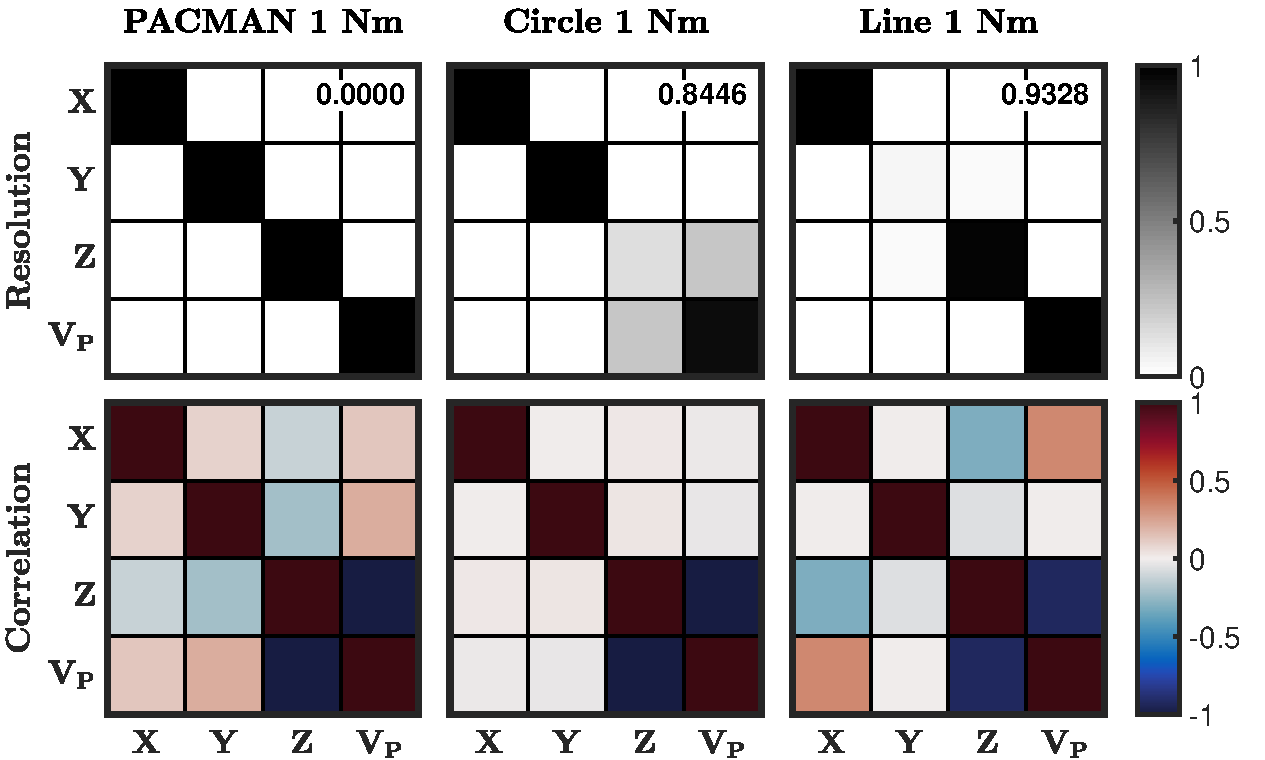
\includegraphics[trim=0cm 0cm 0cm 0cm,clip=true,width=\columnwidth]{Figure07.pdf}
\caption{ Model resolution and correlation matrices for 3 survey configurations of radius 1 Nm: (left) \textit{PACMAN}, (center) \textit{Circle}, and (right) \textit{Line}. The \textit{Line} survey is parallel to the x-direction. $\text{spread}(\mathbf{R})$ is listed at the top right of each resolution matrix. A spread of zero signifies good model resolution for all parameters.}
\label{fig:resolution_correlation}
\end{figure}

\newpage

%% Example real station - survey pattern + residuals
\begin{figure}[h]
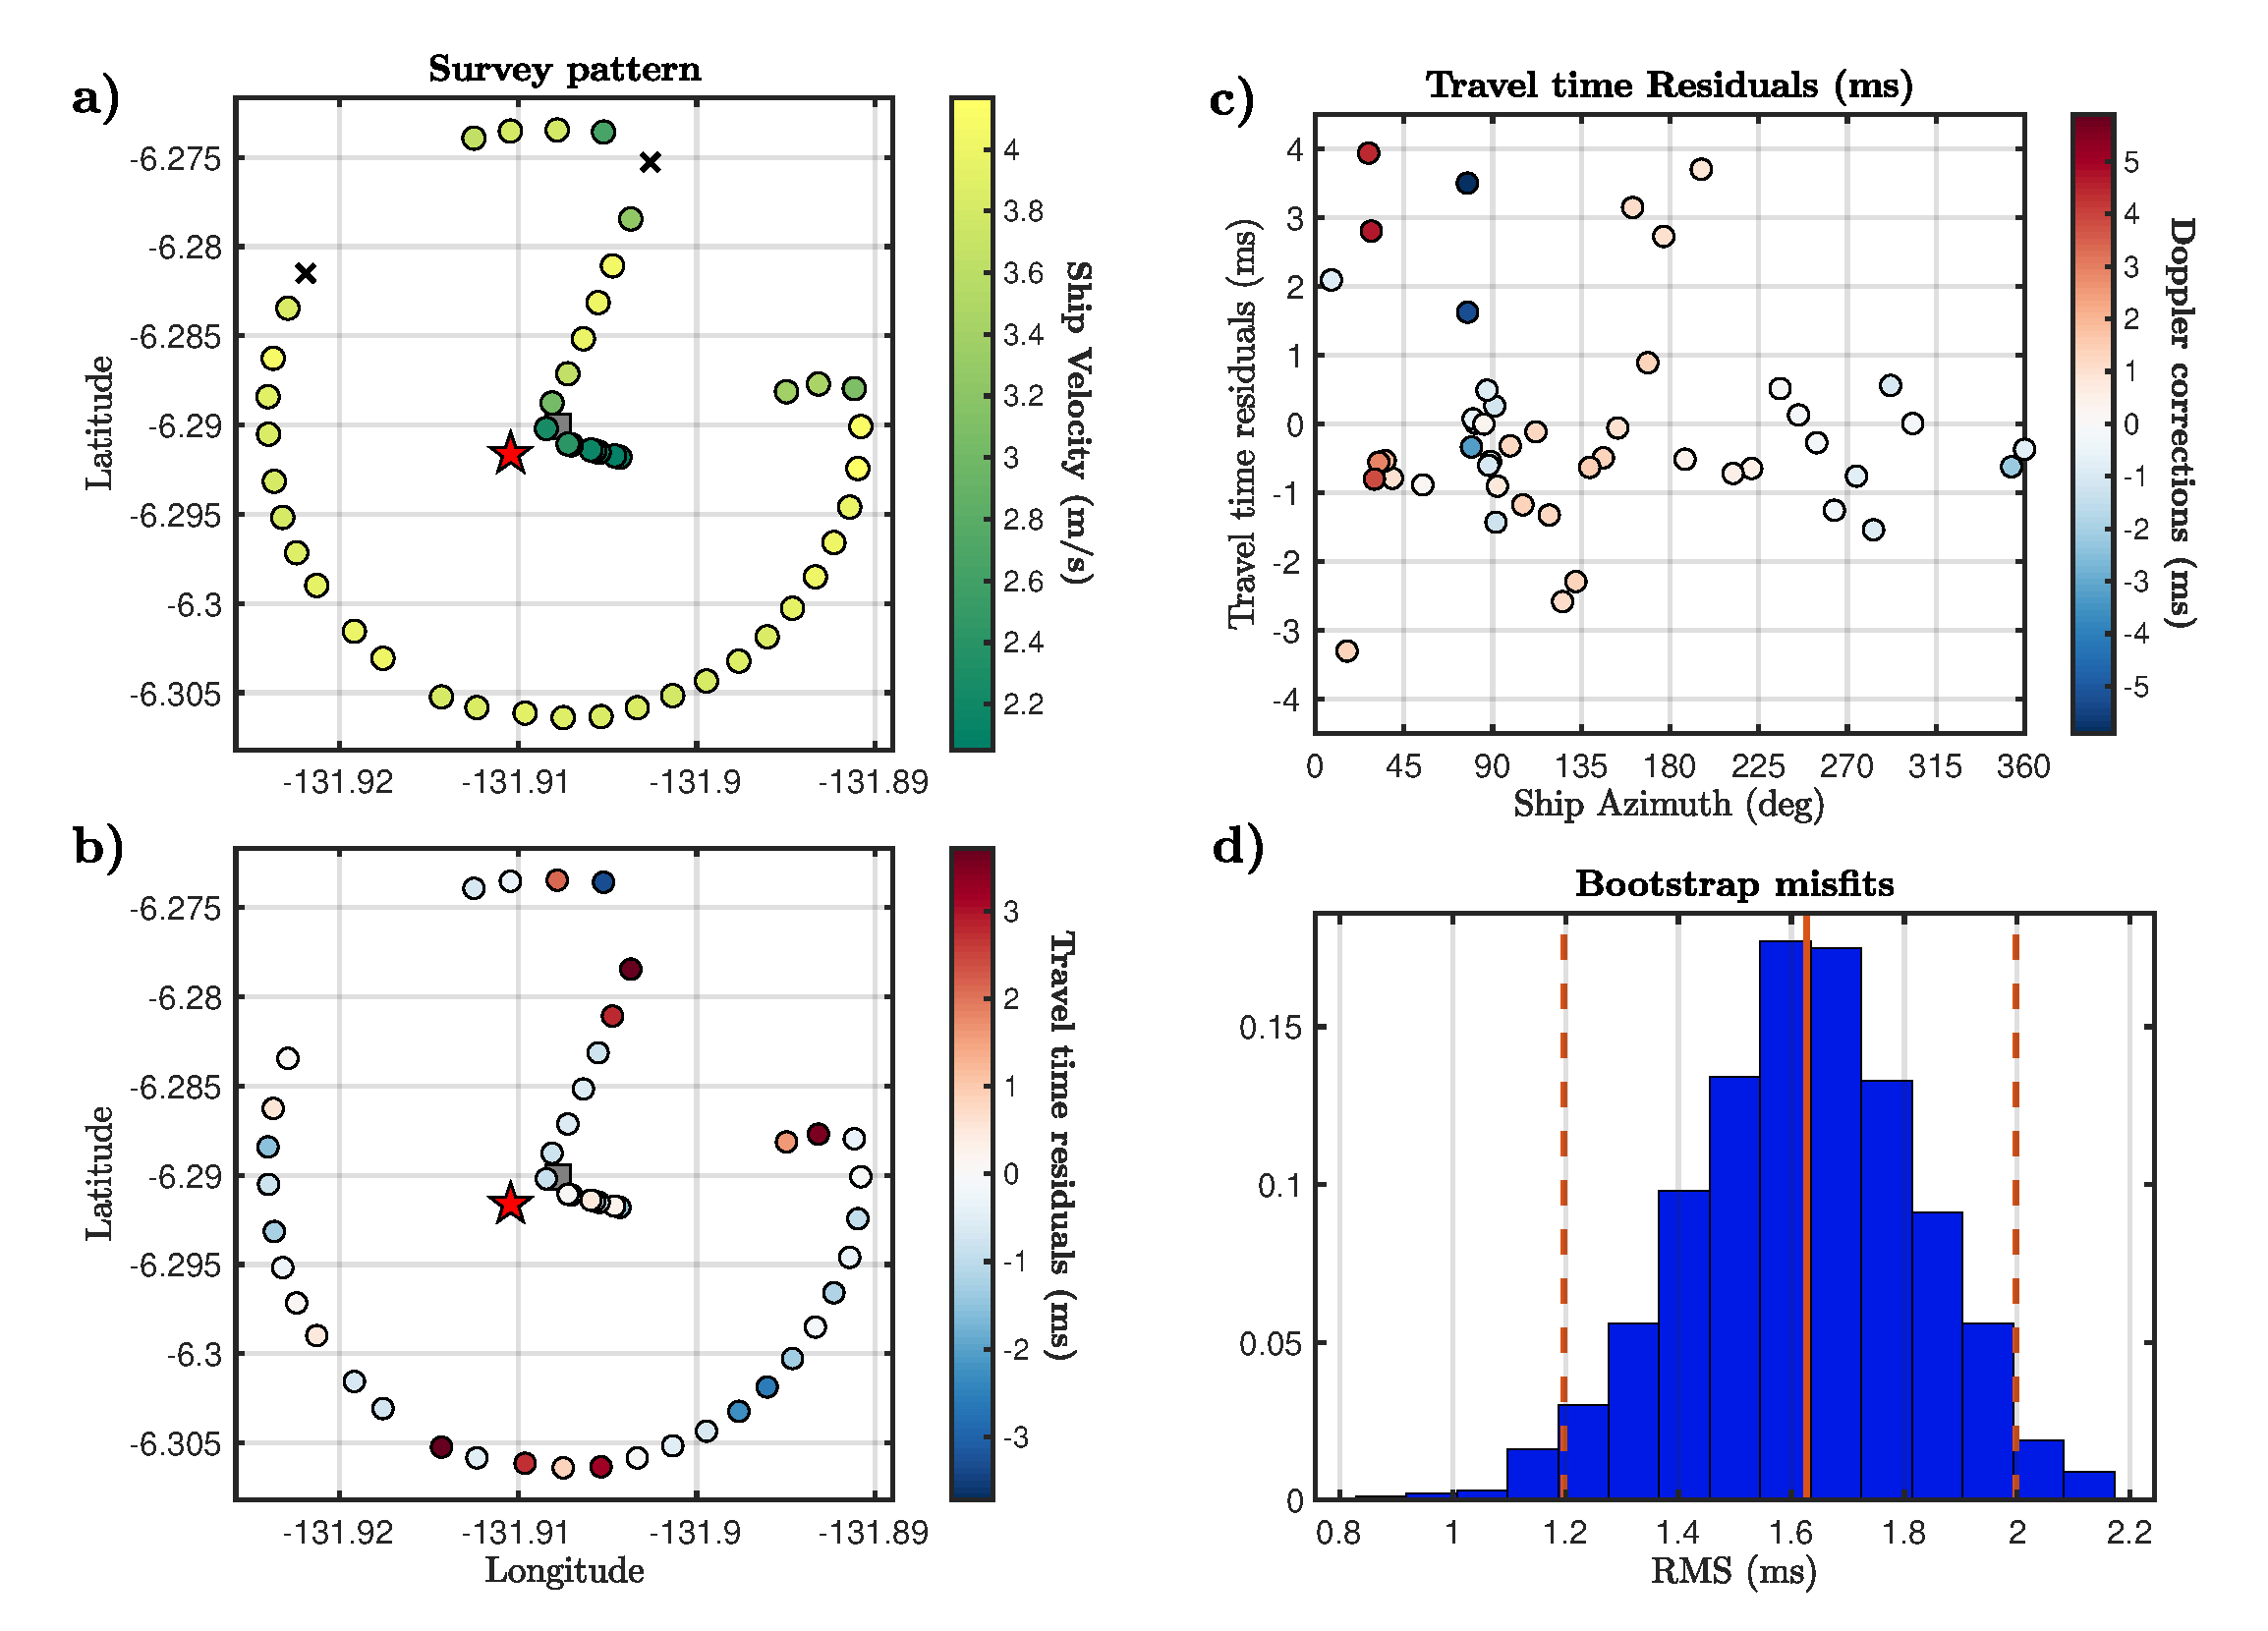
\includegraphics[trim=0cm 0cm 0cm 0cm,clip=true,width=\columnwidth]{Figure02.pdf}
\caption{Example inversion at station EC03 in the 2018 Young Pacific ORCA deployment. a) Map view of acoustic survey; colored circles are successful acoustic range measurements, black crosses are bad measurements rejected by automatic quality control (greater than 500~ms from predicted travel time), gray square is drop location, red star is final location. b) Map view of data residuals based on travel times computed using bootstrap mean station location. c) Data residuals plotted as a function of azimuth, colored by the computed Doppler correction (not used in this inversion). d) Histogram of data RMS from the bootstrap; the RMS of the final model is shown as a red star.}
\label{fig:one_sta_real_survey}
\end{figure}

\newpage

%% Example real station - bootstrap histogram
\begin{figure}[h]
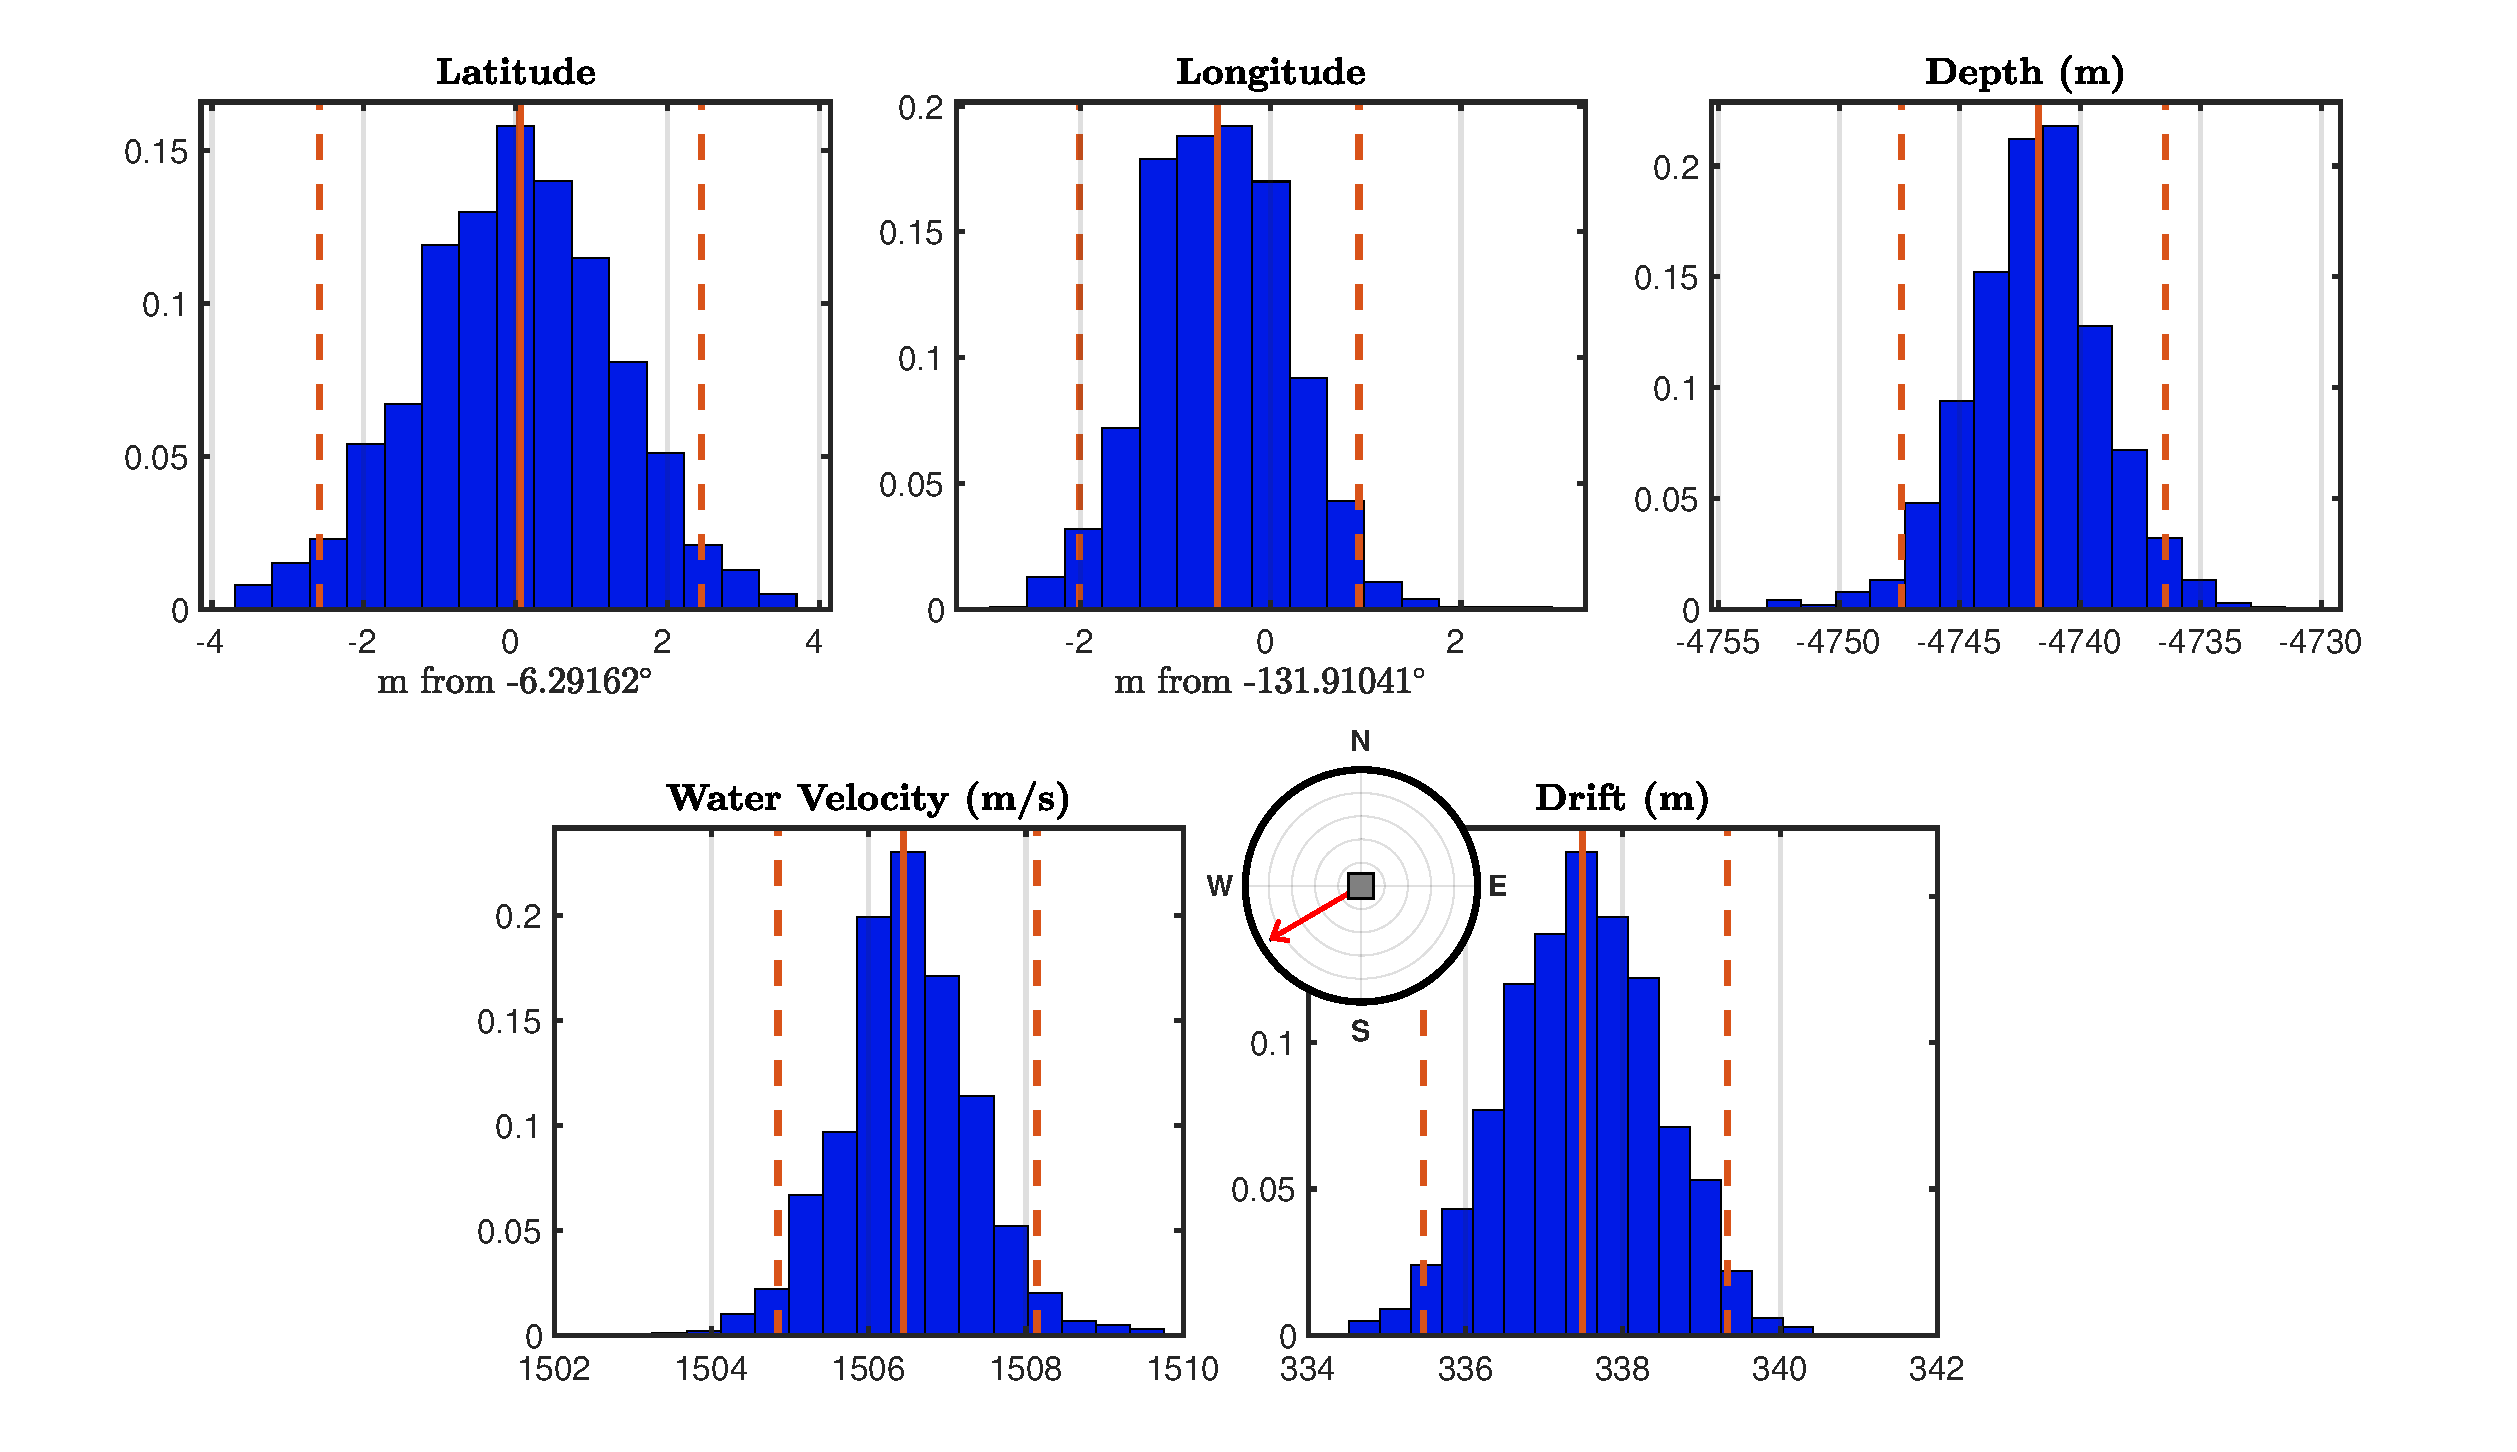
\includegraphics[trim=0cm 0cm 0cm 0cm,clip=true,width=\columnwidth]{Figure03.pdf}
\caption{Histograms of model parameters from the bootstrap inversion of station EC03 in the 2018 Young Pacific ORCA deployment. Red solid line shows mean value, while dashed lines indicate 95th percentiles. Latitude and longitude are plotted in meters from the mean point, for ease of interpretation. The inset plot shows the mean drift azimuth from the drop location (gray square).}
\label{fig:one_sta_real_histograms}
\end{figure}

\newpage

%% Example real station - F-tests
\begin{figure}[h]
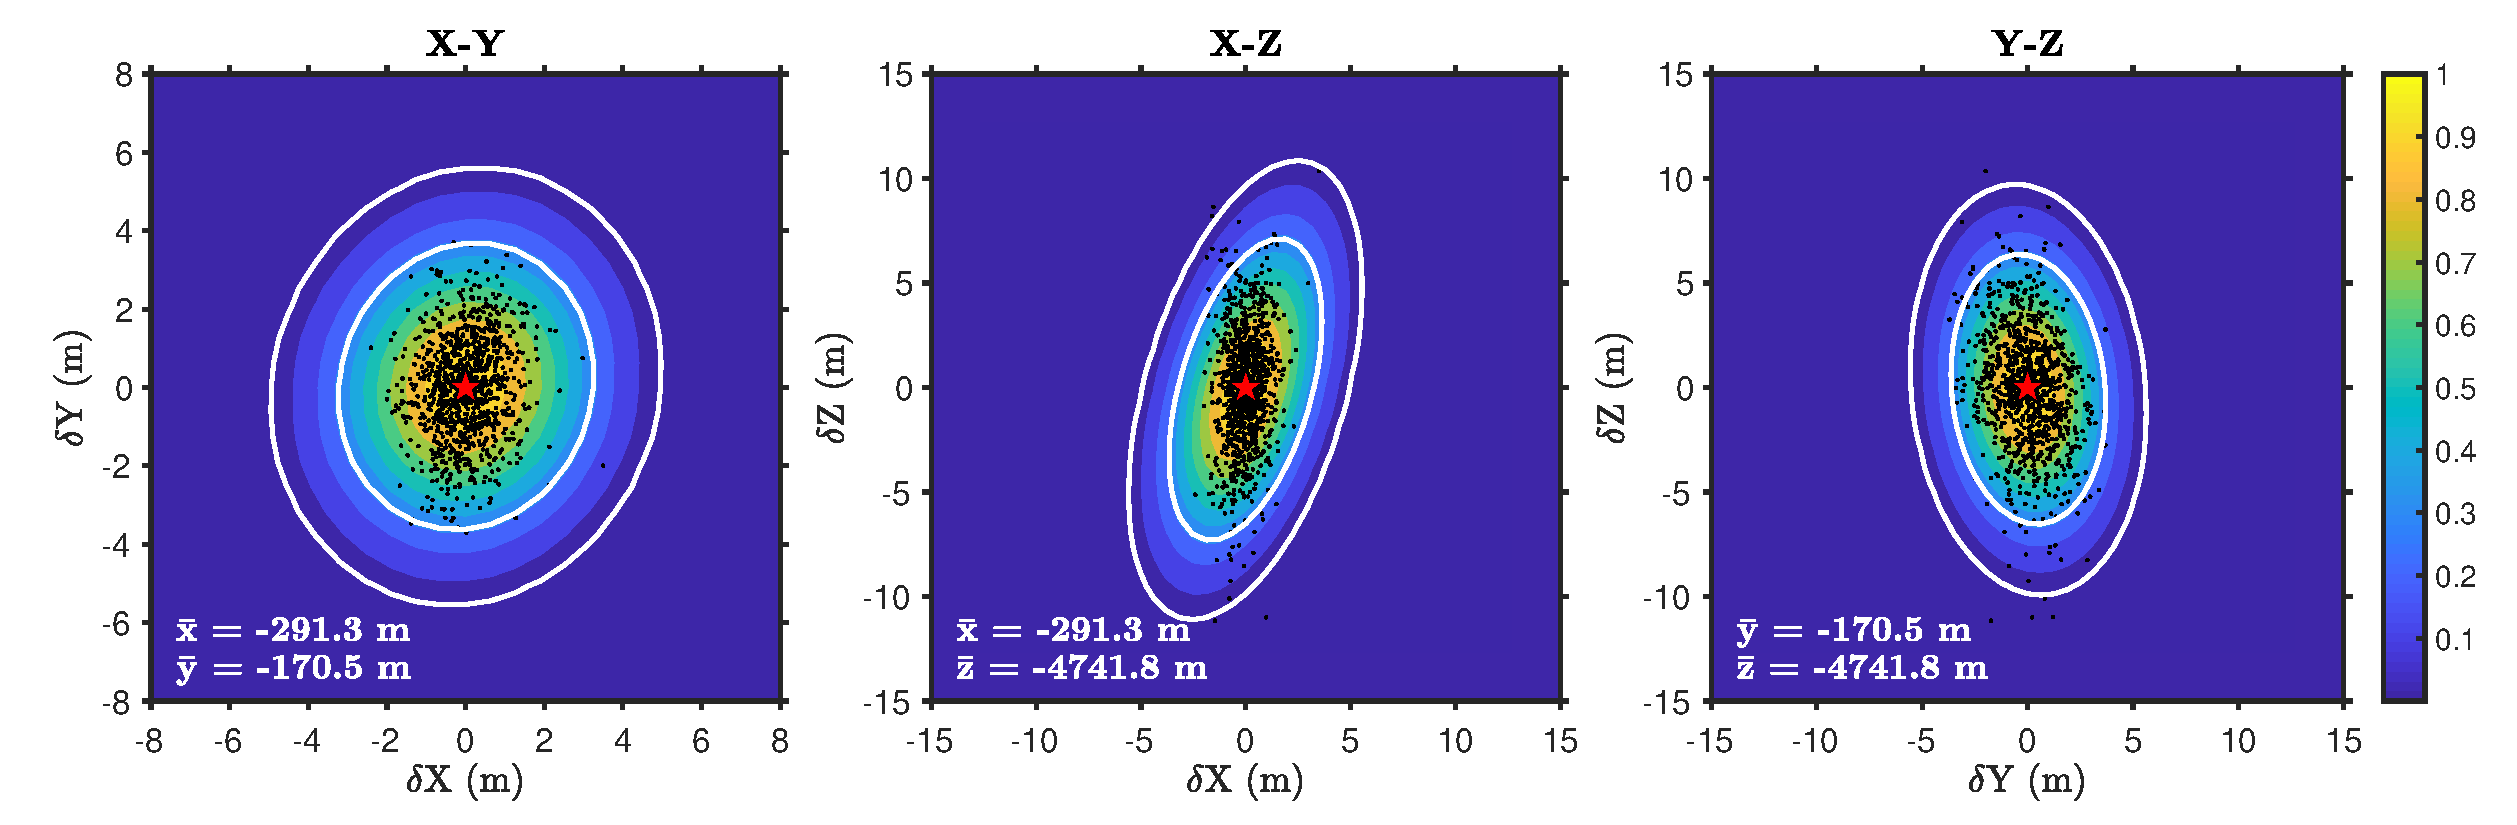
\includegraphics[trim=0cm 0cm 0cm 0cm,clip=true,width=\columnwidth]{Figure04.pdf}
\caption{ Three orthogonal slices through the F-test probability volume for station EC03 in the 2018 Young Pacific ORCA deployment, contoured by probability of true station location relative to the best fitting inverted location ($\bar{x},\bar{y},\bar{z}$), indicated by the red star. White contours show 68\% and 95\% contours. Black dots show individual locations from the bootstrap analysis (Figure~\ref{fig:one_sta_real_histograms}).}
\label{fig:one_sta_real_ftests}
\end{figure}

\newpage

%% All stations meso eddy
\begin{figure}[h]
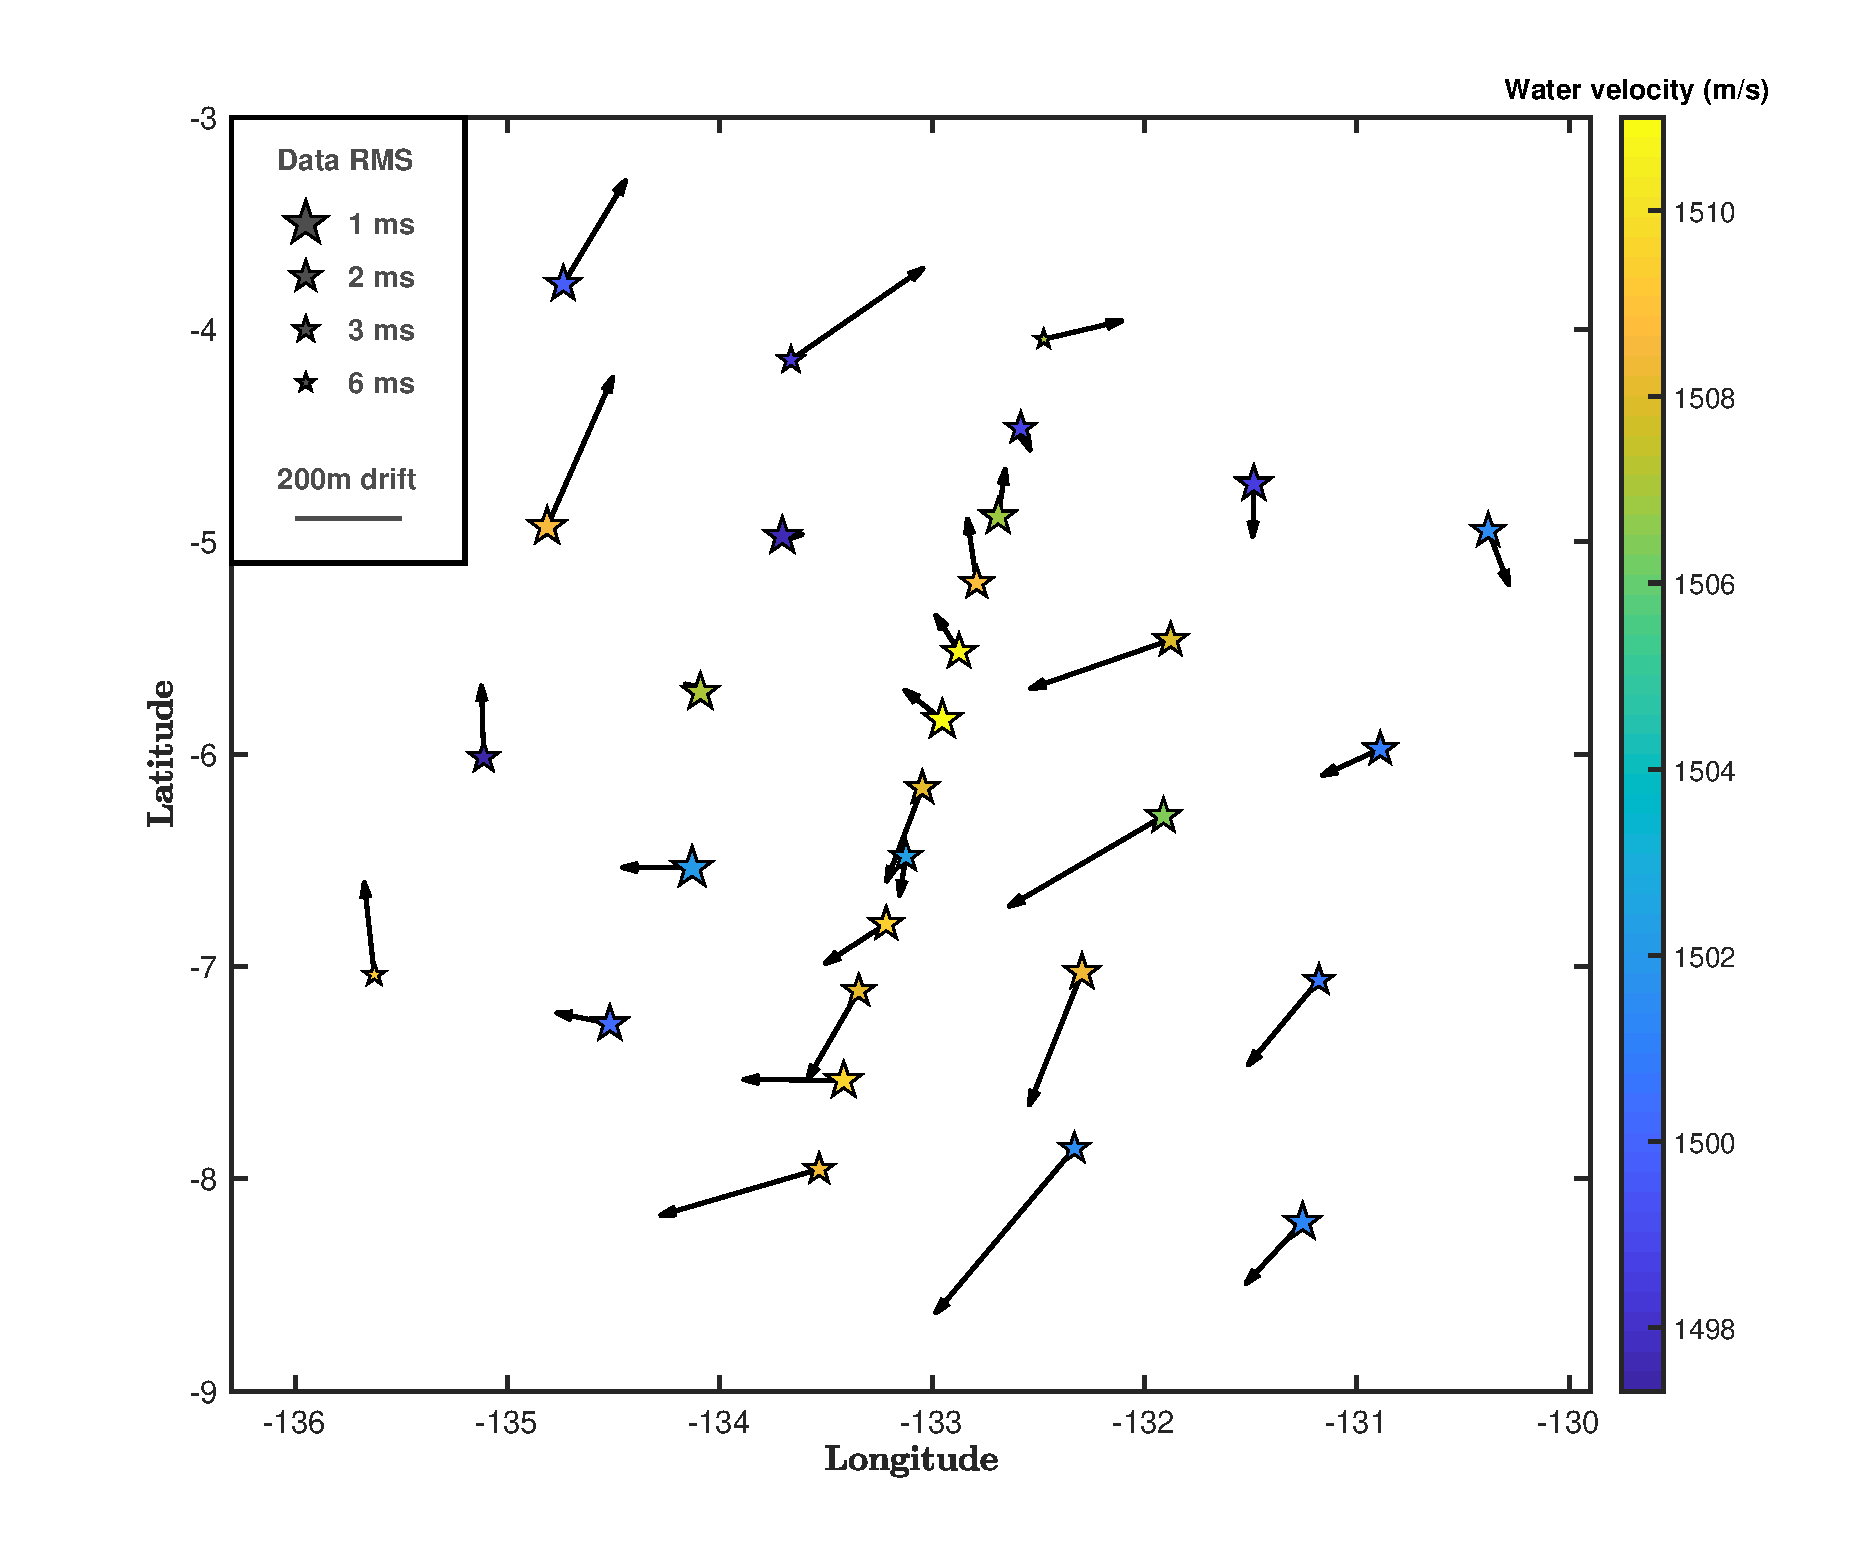
\includegraphics[trim=0cm 0cm 0cm 0cm,clip=true,width=\columnwidth]{Figure08.pdf}
\caption{Pacific ORCA deployment, showing drift directions and magnitudes of each OBS instrument relative to their drop points, as well as the water velocity at each location. Note that drift arrows are not to geographic scale. The systematic clock-wise pattern of drift within the water column resembles a meso-scale cyclonic feature moving through this region approximately during the deployment (see Figure~S1, available in the electronic supplement to this article). Station symbol sizes are inversely scaled to acoustic travel time data misfit.}
\label{fig:meso_eddy}
\end{figure}